% Rebuild the PDF from this directory (run pdflatex twice to settle citations):
%   pdflatex -synctex=0 -jobname=Winter_Bells_Lab_Instructions -interaction=nonstopmode -halt-on-error winter_bells_lab_instructions.tex
%   pdflatex -synctex=0 -jobname=Winter_Bells_Lab_Instructions -interaction=nonstopmode -halt-on-error winter_bells_lab_instructions.tex
% After checking the PDF, remove the generated auxiliary files:
%   PowerShell: Remove-Item Winter_Bells_Lab_Instructions.aux, Winter_Bells_Lab_Instructions.log, Winter_Bells_Lab_Instructions.out -ErrorAction SilentlyContinue
%   Bash:       rm -f Winter_Bells_Lab_Instructions.aux Winter_Bells_Lab_Instructions.log Winter_Bells_Lab_Instructions.out
\documentclass[12pt]{article}
\usepackage[T1]{fontenc}
\usepackage[utf8]{inputenc}
\usepackage{hyperref}
\usepackage[most]{tcolorbox}
\usepackage{graphicx}
\usepackage{array}
\usepackage{geometry}
\usepackage{listings}
\usepackage{xcolor}
\usepackage{cite}
\usepackage{booktabs}
\usepackage{needspace}
\geometry{margin=0.85in}
\linespread{1.06}

\definecolor{UoGMaroon}{HTML}{7A003C}
\definecolor{UoGLight}{HTML}{F7EEF2}
\definecolor{UoGDark}{HTML}{4A0023}
\definecolor{codeblue}{rgb}{0.13,0.29,0.53}

\hypersetup{colorlinks=true,urlcolor=codeblue,citecolor=UoGMaroon}
\urlstyle{same}

\lstset{
  basicstyle=\color{blue}\ttfamily\small,
  keywordstyle=\color{blue}\ttfamily\small,
  commentstyle=\color{gray}\ttfamily\small,
  stringstyle=\color{red}\ttfamily\small,
  breaklines=true
}

\title{\Large\textbf{Raspberry Pi Winter Bells Lab}\\[0.5ex]
\large A hands-on introduction to the Sense HAT, pixel art and sound}
\author{School of Computer Science -- Computing Systems, University of Galway}
\date{November 2026}

\begin{document}

\begin{center}
  
\includegraphics[width=0.32\textwidth]{UOG_LOGO.png}\\[1.5ex]
  {\Large\textbf{University of Galway}}\\[0.8ex]
  {\normalsize School of Computer Science -- Computing Systems}
\end{center}
\vspace{0.8em}
\maketitle

\section*{The Sense HAT - a sensing module for Raspberry pi}
The photo shows the Sense HAT in its usual place: directly on the Raspberry Pi's 40-pin GPIO header. Its name is short for ``Hardware Attached on Top''. The board turns a Pi into a compact, hands-on interface: it can show information, measure its surroundings and respond to a person's input.

The display is an 8$\times$8 grid of 64 RGB LEDs. Each pixel mixes red, green and blue light; each colour value runs from 0 (off) to 255 (brightest). You can use the grid as a tiny canvas for a scrolling message, a pixel-art picture or an animation. It can also make readings visible: for example, a row of lit pixels could show a changing temperature.

The small joystick provides five directions of input---up, down, left, right and press---so a project can react to its user. The sensors add another kind of input. The board measures temperature, humidity and air pressure, and its accelerometer, gyroscope and magnetometer detect movement and orientation. In other words, the Sense HAT can help a Pi notice both what is happening around it and how it is being moved \cite{sensehat}.

\begin{center}
  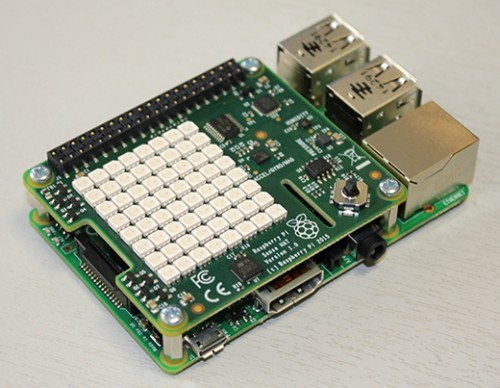
\includegraphics[width=0.92\linewidth,height=7.2cm,keepaspectratio]{sense_hat_on_pi.png}\\[3pt]
  {\small\itshape The Sense HAT mounted on a Raspberry Pi. Photograph: Raspberry Pi Foundation \cite{sensehat-photo}.}
\end{center}

We will spend this lab with the LED display and sound, rather than trying every sensor. As you work, keep an eye out for ideas you could return to in Semester 2 or at the hackathon.

\begin{tcolorbox}[colback=UoGLight,colframe=UoGMaroon,title=The Sense HAT in space]
The board has a space connection. Astro Pi Mission Space Lab invites student teams to collect data with computers aboard the ISS, and the 2025/26 challenge confirms that student programs are still being run there \cite{astro-mission,astropi-current}. The Raspberry Pi Foundation has reported the Sense HAT-equipped Astro Pi units in ESA's Columbus laboratory \cite{astropi-location}; NASA describes Columbus as a research module on the station \cite{nasa-columbus}. That is the reported location of the flight units, not a claim that the hardware never moves. The board on your desk is, of course, staying on Earth.
\end{tcolorbox}

For an optional maker extension, the Raspberry Pi Foundation has also published 3D-printable parts for an Astro Pi flight-case model. It is a project enclosure, not a flight-qualified case \cite{astro-flight-case}.

\section*{What You Will Take Away}
By the end of the session, you should have a feel for:
\begin{itemize}
  \item How the Sense HAT's display is programmed, we will study more in semester 02.
  \item How to produce musical tones, we will study more on it in semester 02.
  \item What projects can I develop with a PI and a sensehat for the hackathon challange.
\end{itemize}

\Needspace{0.6\textheight}
\section*{What's in Your Lab Pack?}
Start with \texttt{README.txt} for the task steps; the table lists the rest of the pack.

\small
\setlength{\tabcolsep}{3pt}
\renewcommand{\arraystretch}{0.94}
\begin{tabular}{p{0.42\linewidth}p{0.51\linewidth}}
\toprule
\textbf{File} & \textbf{What it is for} \\
\midrule
\texttt{README.txt} & Task steps and troubleshooting. \\
\texttt{setup\_pi.sh} & Checks lab libraries and editors. \\
\texttt{task1\_verify.py} & Checks the Sense HAT with one LED. \\
\texttt{task2\_display\_and\_art.py} & Scrolling message and 64-pixel art. \\
\texttt{pixel\_studio\_gui.py} & Pixel Studio with seven presets. \\
\texttt{task3\_music\_tones.py} & NumPy bell tones and rhythms. \\
\texttt{task4\_winter\_bells\_symphony.py} & Combines the display and music. \\
\texttt{solutions.zip} & Completed scripts for all tasks. \\
\bottomrule
\end{tabular}
\normalsize

\section*{Pre-Task: Shell Environment Setup}
Before starting, extract the lab folder on the Raspberry Pi. Open a terminal, move into \texttt{winter\_bells\_lab}, and run:
\begin{lstlisting}
cd ~/winter_bells_lab
chmod +x setup_pi.sh
./setup_pi.sh
\end{lstlisting}
Check that \texttt{sense\_hat}, \texttt{pygame}, \texttt{numpy} and \texttt{tkinter} report as ready. Then open the task files in Thonny or Geany. If you use Geany, set its Execute command to \texttt{python3 "\%f"}. The comments in the scripts explain how the hardware and sounds work; look for the TODOs where you can make them your own.

\section*{Lab Task}
\begin{tcolorbox}[colback=UoGLight,colframe=UoGMaroon,title=The Sense HAT in space]
\begin{enumerate}
  \item \textbf{First, meet the hardware  -- \texttt{task1\_verify.py}.} Run the short check and look for the single gold LED. This confirms that the Pi can talk to the Sense HAT; there is no music or scrolling display activity yet.
  \item \textbf{Try to print on display  -- \texttt{task2\_display\_and\_art.py}.} Give the Sense HAT a greeting of your own, then open Pixel Studio. Start from one of its seven presets---Winter Bell, Bell, Snowflake, Winter Star, Snowman, Winter Pine or Winter Frost Pattern---or draw your own. Paste the resulting 64-pixel list into TODO 2 and run the script to see your design on the physical display.
  \item \textbf{Then, make a sound of your own  -- \texttt{task3\_music\_tones.py}.} This task is about sound. Listen to the default 116 BPM tune, then try a gentler 100 BPM or a livelier 132 BPM. Choose a melody from the built-in bank, then change pitches and beat lengths to make it your own. The comments explain how NumPy samples a sine wave, how its frequency sets pitch, and how BPM and beat counts determine note duration.
  \item \textbf{Finally, bring it all together  -- \texttt{task4\_winter\_bells\_symphony.py}.} Reuse ideas from the display and music tasks: change the melody sections, add to the snow scene or reuse your pixel art, and write the closing message. Then see if your group can make each light scene feel distinct---and let another group guess which scene is playing.
\end{enumerate}
\end{tcolorbox}
\section*{What to submit}
Take a video of the project and upload it on the canvas

\begin{thebibliography}{9}
\small
\bibitem{sensehat}
Raspberry Pi Ltd., ``Raspberry Pi Sense HAT documentation,'' hardware features and Python library.
\url{https://www.raspberrypi.com/documentation/accessories/sense-hat.html}
(accessed 24 November 2026).

\bibitem{sensehat-photo}
Raspberry Pi Foundation, ``The Sense HAT: headgear for the terminally curious,'' 13 May 2015.
\url{https://www.raspberrypi.org/blog/the-sense-hat-headgear-for-the-terminally-curious/}
Photograph:
\url{https://www.raspberrypi.org/wp-content/uploads/2015/05/sense-hat.jpg}
(accessed 24 November 2026).

\bibitem{astropi-location}
Raspberry Pi Foundation, ``Astro Pi upgrades on the International Space Station,'' 19 September 2017.
\url{https://www.raspberrypi.org/blog/astro-pi-upgrades/}
(reports the Astro Pi units in the Columbus module; accessed 24 November 2026).

\bibitem{astropi-current}
European Space Agency, ``A stellar milestone: Astro Pi programs on their way to the ISS,'' 22 April 2026.
\url{https://www.esa.int/Education/AstroPI/A_stellar_milestone_Astro_Pi_programs_on_their_way_to_the_ISS}
(2025/2026 Astro Pi challenge update; accessed 24 November 2026).

\bibitem{astro-mission}
Astro Pi, ``Mission Space Lab,'' current programme overview.
\url{https://astro-pi.org/mission-space-lab}
(accessed 24 November 2026).

\bibitem{nasa-columbus}
NASA, ``Columbus Laboratory Module,'' International Space Station.
\url{https://www.nasa.gov/international-space-station/columbus-laboratory-module/}
(accessed 24 November 2026).

\bibitem{astro-flight-case}
Raspberry Pi Foundation, ``Astro Pi: 3D-Print Your Own Flight Case,'' 8 February 2016.
\url{https://www.raspberrypi.org/blog/astro-pi-3d-print-your-own-flight-case/}
(accessed 24 November 2026).

\bibitem{google-ai-studio}
Google, \emph{Google AI Studio}, AI tool used to assist in preparing this lab handout.
\url{https://aistudio.google.com/} (accessed 24 November 2026).
\end{thebibliography}

\end{document}
